\ifx\wholebook\relax \else
% ------------------------

\documentclass[b5paper]{article}
\usepackage[nomarginpar
  %, margin=.5in
]{geometry}

\addtolength{\oddsidemargin}{-0.05in}
\addtolength{\evensidemargin}{-0.05in}
\addtolength{\textwidth}{0.1in}

\usepackage[en]{../../prelude}

\setcounter{page}{1}

\begin{document}

\title{Insertion sort}

\author{Xinyu LIU
\thanks{{\bfseries Xinyu LIU} \newline
  Email: liuxinyu95@gmail.com \newline}
  }

\maketitle
\fi

\markboth{Insertion sort}{Elementary Algorithms}

\ifx\wholebook\relax
\chapter{Insertion sort}
\numberwithin{Exercise}{chapter}
\fi

\section{Introduction}
\label{sec:isort-introduction} \index{insertion sort}

Insertion sort is a straightforward sort algorithm\footnote{We skip the `Bubble sort' method\cite{wiki-bubble-sort}.}. We give its preliminary definition in chapter 1. For a collection of comparable elements, we repeatedly pick one, insert them to a list and maintain the ordering. As every insertion takes linear time, its performance is bound to $O(n)$ where $n$ is the number of elements. This performance is not as good as the divide and conqueror sort algorithms, like quick sort and merge sort. However, we can still find its application today. For example, a well tuned quick sort implementation falls back to insertion sort for small data set. The idea of insertion sort is as same as sorting a deck of a poker cards\cite{CLRS}. The cards are shuffled. A player takes card one by one. At any time, all cards on hand are sorted. When gets a new card, the player inserts it in proper position according to the order of points as shown in figure \ref{fig:hand-of-cards}.

\begin{figure}[htbp]
  \centering
  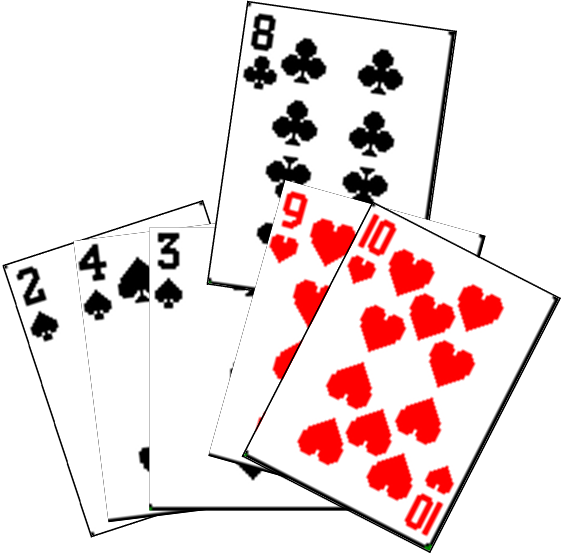
\includegraphics[scale=0.5]{img/card-deck.png}
  \caption{Insert card 8 to a deck.}
  \label{fig:hand-of-cards}
\end{figure}

Based on this idea, we can implement insertion sort as below:

\begin{algorithmic}[1]
\Function{Sort}{$A$}
  \State $S \gets$ NIL
  \For{each $a \in A$}
    \State \Call{Insert}{$a, S$}
  \EndFor
  \State \Return $S$
\EndFunction
\end{algorithmic}

Or define it with $fold_l$ in Curried form:

\be
sort = fold_l(insert, \nil)
\ee

We store the sorted result in a new array, alternatively, we can change it to in-place:

\begin{algorithmic}[1]
\Function{Sort}{$A$}
  \For{$i \gets 2$ to $|A|$}
    \State ordered insert $A[i]$ to $A[1...(i-1)]$
  \EndFor
\EndFunction
\end{algorithmic}

Where the index $i$ ranges from 1 to $n = |A|$. We start from 2, because the singleton sub-array $[A[1]]$ is ordered. When process the $i$-th element, all elements before $i$ are sorted. We continuously insert elements till consume all the unsorted ones, as shown in figure \ref{fig:in-place-sort}.

\begin{figure}[htbp]
  \centering
  \includegraphics[scale=0.8]{img/in-place-sort.ps}
  \caption{Continuously insert elements to the sorted part.}
  \label{fig:in-place-sort}
\end{figure}

We can also define $sort$ recursively:

\be
\begin{array}{rcl}
sort(\nil) & = & \nil \\
sort(x:xs) & = & insert(x, sort(xs)) \\
\end{array}
\ee

\section{Insertion}
\index{insertion sort!insertion}

In chapter 1, we give the ordered insertion algorithm for list. For array, we can also scan it to locate the insert position. We can either scan from left or right. Below algorithm is from right:

\begin{algorithmic}[1]
\Function{Sort}{$A$}
  \For{$i \gets 2$ to $|A|$}
    \Comment{Insert $A[i]$ to $A[1...(i-1)]$}
    \State $x \gets A[i]$
    \State $j \gets i-1$
    \While{$j > 0$ and $x < A[j]$ }
      \State $A[j+1] \gets A[j]$
      \State $j \gets j - 1$
    \EndWhile
    \State $A[j+1] \gets x$
  \EndFor
\EndFunction
\end{algorithmic}

It's expensive to insert at arbitrary position, as array stores elements continuously. When insert $x$ at position $i$, we need shift all elements after $i$ (i.e. $i + 1, i + 2, ...$) one cell to right. After free the cell at $i$, we put $x$ in, as shown in figure \ref{fig:array-shift}.

\begin{figure}[htbp]
  \centering
  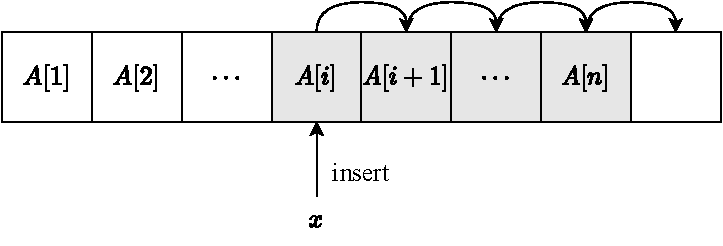
\includegraphics[scale=0.7]{img/array-shift.ps}
  \caption{Insert $x$ to $A$ at $i$.}
  \label{fig:array-shift}
\end{figure}

For the array of length $n$, suppose after comparing $x$ to the first $i$ elements, we located the position to insert. Then we shift the rest $n - i + 1$ elements, and put $x$ in the $i$-th cell. Overall, we need traverse the whole array if scan from left. On the other hand, if scan from right to left, we examine $n - i + 1$ elements, and perform the same amount of shifts. We can also define a separated \textproc{Insert}() function, and call it inside the loop. The insertion takes linear time no matter scans from left or right, hence the sort algorithm is bound to $O(n^2)$, where $n$ is the number of elements.

\begin{Exercise}
\Question{Implement the insert to scan from left to right.}
\Question{Define the insert function, and call it from the sort algorithm.}
\end{Exercise}

\section{Binary search}
\index{Insertion sort!binary search}

When insert a poker card, we don't scan, but take a quick glance at the deck to locate the position. We can do this because the deck is sorted. Binary search is such a method that applies to ordered sequence.

\begin{algorithmic}[1]
\Function{Sort}{$A$}
  \For{$i \gets 2$ to $|A|$}
    \State $x \gets A[i]$
    \State $p \gets $ \Call{Binary-Search}{$x, A[1...(i-1)]$}
    \For{$j \gets i$ down to $p$}
      \State $A[j] \gets A[j-1]$
    \EndFor
    \State $A[p] \gets x$
  \EndFor
\EndFunction
\end{algorithmic}

Binary search utilize the fact that the slice $A[1...(i-1)]$ is ordered. Suppose it is ascending without loss of generality (as we can define $\leq$ abstract). To find the position $j$ that satisfies $A[j-1] \leq x \leq A[j]$, we compare $x$ to the middle element $A[m]$, where $m = \lfloor \dfrac{i}{2} \rfloor$. If $x < A[m]$, we then recursively apply binary search to the first half; otherwise, we search the second half. As every time, we halve the elements, binary search takes $O(\lg i)$ time to locate the insertion position.

\begin{algorithmic}[1]
\Function{Binary-Search}{$x, A$}
  \State $l \gets 1, u \gets 1+|A|$
  \While{$l < u$}
    \State $m \gets \lfloor \dfrac{l+u}{2} \rfloor$
    \If{$A[m] = x$}
      \State \Return $m$ \Comment{Duplicated element}
    \ElsIf{$A[m] < x$}
      \State $l \gets m+1$
    \Else
      \State $u \gets m$
    \EndIf
  \EndWhile
  \State \Return $l$
\EndFunction
\end{algorithmic}

The improved sort algorithm is still bound to $O(n^2)$. The one with scan takes $O(n^2)$ comparisons and $O(n^2)$ shifts, withe binary search, it takes $O(n \lg n)$ comparisons and $O(n^2)$ shifts.

\begin{Exercise}
\Question{Implement the recursive binary search.}
\end{Exercise}

\section{List}
\index{Insertion sort!linked-list setting}

With binary search, although the search time improved to $O(n \lg n)$, the shifts are still $O(n^2)$. This is because we need shift array cells when insert, which is linear time. On the other hand, when use list, the insertion is constant time at a given node reference. Below is the list insertion algorithm defined in chapter 1:

\be
\begin{array}{rcl}
insert(x,\ \nil) & = & [x] \\
insert(x,\ y : ys) & = & \begin{cases}
  x \leq y : & x : y : ys \\
  otherwise : & y : insert(x, ys) \\
  \end{cases}
\end{array}
\ee

Translating the algorithm to Haskell yields the below program.

\lstset{language=Haskell}
\begin{lstlisting}
insert [] x = [x]
insert (y:ys) x = if x < y then x:y:ys else y:insert ys x
\end{lstlisting}

And we can complete the two versions of insertion sort program based on
the first two equations in this chapter.

\begin{lstlisting}
isort [] = []
isort (x:xs) = insert (isort xs) x
\end{lstlisting}

Or we can represent the recursion with folding.

\begin{lstlisting}
isort = foldl insert []
\end{lstlisting}

Linked-list setting solution can also be described imperatively. Suppose
function \textproc{Key}($x$), returns the value of element stored in node
$x$, and \textproc{Next}($x$) accesses the next node in the linked-list.

\begin{algorithmic}
\Function{Insert}{$L, x$}
  \State $p \gets$ NIL
  \State $H \gets L$
  \While{$L \neq$ NIL $\land $ \Call{Key}{$L$} $<$ \Call{Key}{$x$}}
    \State $p \gets L$
    \State $L \gets $ \Call{Next}{$L$}
  \EndWhile
  \State \Call{Next}{$x$} $\gets L$
  \If{$p =$ NIL}
    \State $H \gets x$
  \Else
    \State \Call{Next}{$p$} $\gets x$
  \EndIf
  \State \Return $H$
\EndFunction
\end{algorithmic}

For example in ANSI C, the linked-list can be defined as the following.

\lstset{language=C}
\begin{lstlisting}
struct node{
  Key key;
  struct node* next;
};
\end{lstlisting}

Thus the insert function can be given as below.

\begin{lstlisting}
struct node* insert(struct node* lst, struct node* x){
  struct node *p, *head;
  p = NULL;
  for(head = lst; lst && x->key > lst->key; lst = lst->next)
    p = lst;
  x->next = lst;
  if(!p)
    return x;
  p->next = x;
  return head;
}
\end{lstlisting}

Instead of using explicit linked-list such as by pointer or reference
based structure. Linked-list can also be realized by another index array.
For any array element $A[i]$, $Next[i]$ stores the index of next element
follows $A[i]$. It means $A[Next[i]]$ is the next element after $A[i]$.

The insertion algorithm based on this solution is given like below.

\begin{algorithmic}
\Function{Insert}{$A, Next, i$}
  \State $j \gets \perp$
  \While{$Next[j] \neq$ NIL $\land A[Next[j]] < A[i]$}
    \State $j \gets Next[j]$
  \EndWhile
  \State $Next[i] \gets Next[j]$
  \State $Next[j] \gets i$
\EndFunction
\end{algorithmic}

Here $\perp$ means the head of the $Next$ table.
And the relative Python program for this algorithm is given as the following.

\lstset{language=Python}
\begin{lstlisting}
def isort(xs):
    n = len(xs)
    next = [-1]*(n+1)
    for i in range(n):
        insert(xs, next, i)
    return next

def insert(xs, next, i):
    j = -1
    while next[j] != -1 and xs[next[j]] < xs[i]:
        j = next[j]
    next[j], next[i] = i, next[j]
\end{lstlisting}

Although we change the insertion operation to constant time by using
linked-list. However, we have to traverse the linked-list to find the
position, which results $O(n^2)$ times comparison. This is because
linked-list, unlike array, doesn't support random access. It means we
can't use binary search with linked-list setting.

\begin{Exercise}
\begin{itemize}
\item Complete the insertion sort by using linked-list insertion function
in your favorate imperative programming language.
\item The index based linked-list return the sequence of rearranged index
as result. Write a program to re-order the original array of elements from
this result.
\end{itemize}
\end{Exercise}

% ================================================================
% Final improvement
% ================================================================

\section{Final improvement by binary search tree}
\index{Insertion sort!binary search tree}

It seems that we drive into a corner. We must improve both the comparison
and the insertion at the same time, or we will end up with $O(n^2)$ performance.

We must use binary search, this is the only way to improve the comparison
time to $O(\lg n)$. On the other hand, we must change the data structure,
because we can't achieve constant time insertion at a position with
plain array.

This remind us about our 'hello world' data structure, binary search tree.
It naturally support binary search from its definition. At the same time,
We can insert a new node in binary search tree in $O(1)$ constant time
if we already find the location.

So the algorithm changes to this.

\begin{algorithmic}
\Function{Sort}{$A$}
  \State $T \gets \phi$
  \For{each $x \in A$}
    \State $T \gets $ \Call{Insert-Tree}{$T, x$}
  \EndFor
  \State \Return \Call{To-List}{$T$}
\EndFunction
\end{algorithmic}

Where \textproc{Insert-Tree}() and \textproc{To-List}() are described in
previous chapter about binary search tree.

As we have analyzed for binary search tree, the performance of tree sort
is bound to $O(n \lg n)$, which is the lower limit of comparison based
sort\cite{Knuth}.

\section{Short summary}
In this chapter, we present the evolution process of insertion sort. Insertion
sort is well explained in most textbooks as the first sorting algorithm.
It has simple and straightforward idea, but the performance is quadratic.
Some textbooks stop here, but we want to show that there exist ways to improve
it by different point of view. We first try to save the comparison time
by using binary search, and then try to save the insertion operation by
changing the data structure to linked-list. Finally, we combine these
two ideas and evolute insertion sort to tree sort.

\begin{thebibliography}{99}

\bibitem{wiki-bubble-sort}
http://en.wikipedia.org/wiki/Bubble\_sort

\bibitem{CLRS}
Thomas H. Cormen, Charles E. Leiserson, Ronald L. Rivest and Clifford Stein.
``Introduction to Algorithms, Second Edition''. ISBN:0262032937. The MIT Press. 2001

\bibitem{Knuth}
Donald E. Knuth. ``The Art of Computer Programming, Volume 3: Sorting and Searching (2nd Edition)''. Addison-Wesley Professional; 2 edition (May 4, 1998) ISBN-10: 0201896850 ISBN-13: 978-0201896855

\end{thebibliography}

\ifx\wholebook\relax\else
\end{document}
\fi
